%!TEX root = DMmidterm.tex

\section{Project}
\label{sec:Project}

%\begin{figure*}[]
%	\begin{center}
%		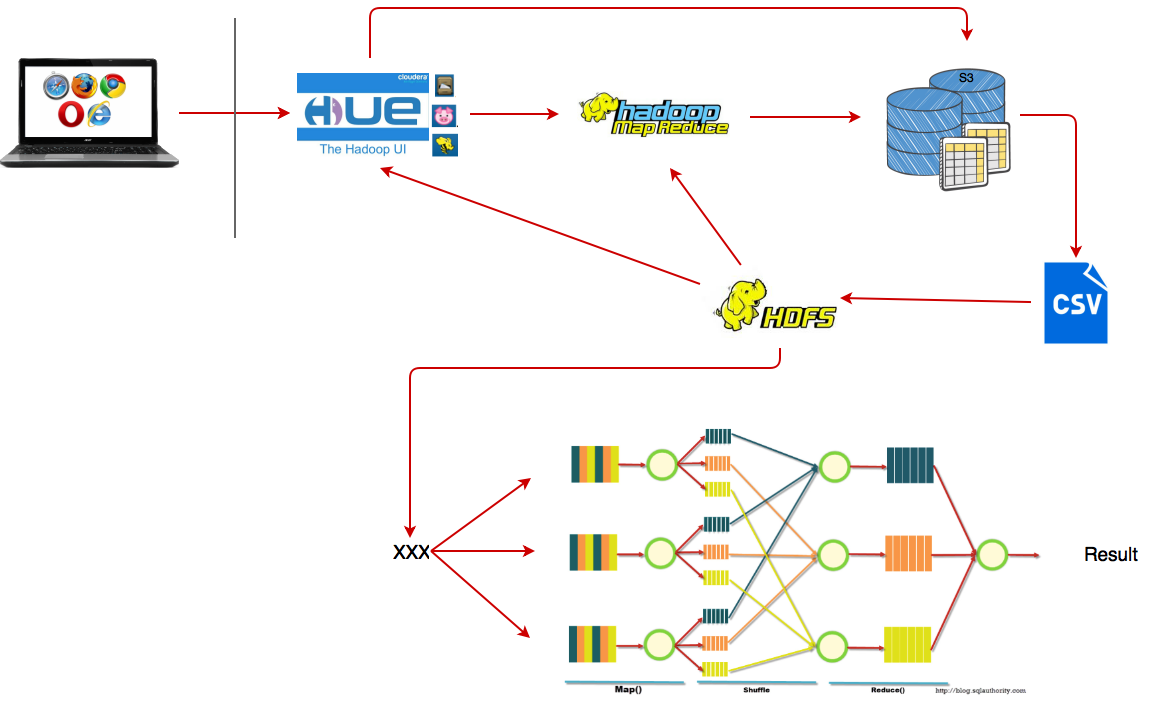
\includegraphics[width=2\columnwidth]{/Users/MariaFerman/Desktop/DC_FinalProject/images/Diagram}
%		\caption{Project Diagram}
%		\label{fig:dataDiagr}
%	\end{center}
%	\vspace{-10pt}
%\end{figure*}

%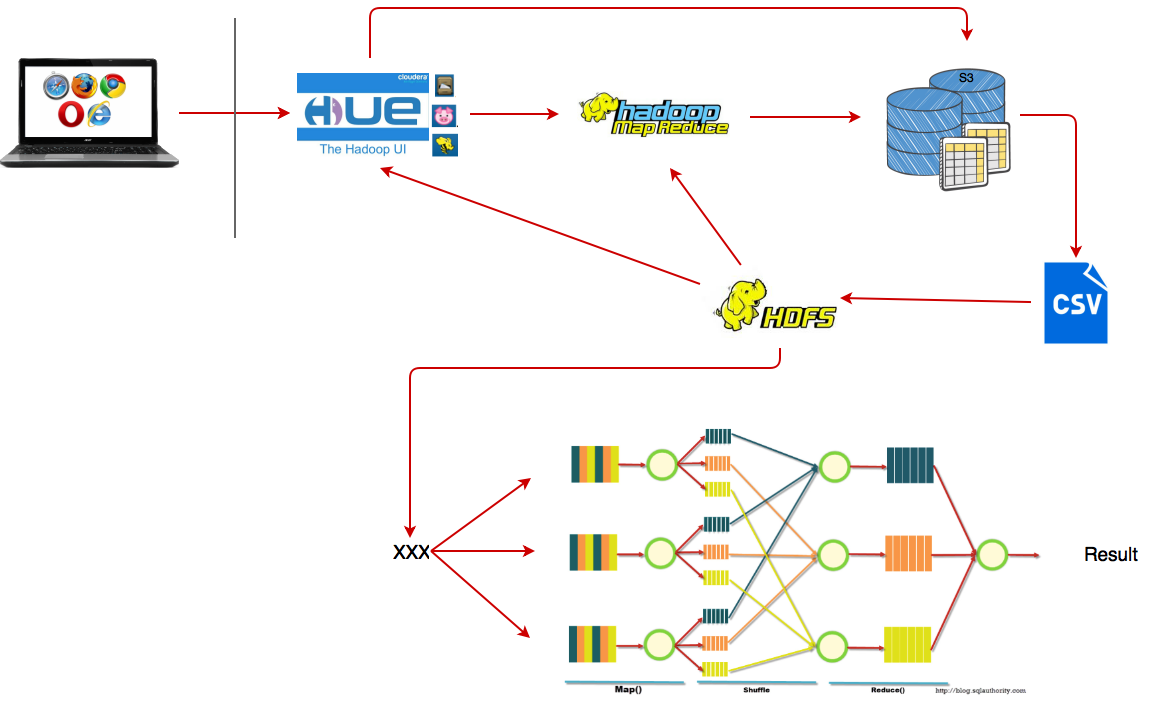
\includegraphics{/Users/MariaFerman/Desktop/DC_FinalProject/images/Diagram}


\subsection{ Dataset}
The dataset gathered for this project comes from the Pacific Climate Impacts Consortium (PCIC) of the University of Vic- toria. The dataset consist in a series of climate measurements that shows how the climate changes and varies over time. All the measurements were gathered at the same location in the Pacific and Yukon region of British Colombia, Canada. The dataset is divided by time and stations. The station is the exact location where the data were gathered. The dataset will allow us to understand the climate change among time and regions (stations). The resulting analysis of the dataset might help for trend analysis and climate change researches. This information can be used as an input for more complex climate models in order to have accurate climate predictions.


\subsection{Scripts}
The project has two main customised scripts for the Hive and Pig process. The first script is for getting the data and the second is for storing and computing the average of the data.

Pig script: This script has several crucial sections. The first one is when the data is extracted from the original CSV file. In the ”raw logs” variable it will be loaded the weblogs into a sequence of tuples.

\begin{lstlisting}
raw_logs =
  LOAD 's3://ds562finalproject/PacificClimate/
  2014_2015_MinTemp/' 
  USING TextLoader AS (line:chararray);
\end{lstlisting}

The second part of the script is for getting the information into the columns ''one\_day\_ precipitation'' for the percentage of precipitation, ''max\_temp'' for the maximum temperature and ''min\_temp'' for the minimum temperature for that specific day. Specifically, it will convert each weblog string into a structure with the above-mentioned columns.

\begin{lstlisting}
logs_base =
  FOREACH  raw_logs
  GENERATE
   FLATTEN (   	 
      EXTRACT(
        line, '^(\\d{4}-\\d{2})-\\d{2} \\d{2}:\\d{2}:\\d{2}, (\\S+), (\\S+), (\\S+)') )
    AS (
      date: chararray, one_day_precipitation: chararray, max_temp: chararray, min_temp: chararray )
\end{lstlisting}

On the next section, the data will be filter in order to separate the dates that have a non-null value. After that, the data will be grouped by the date field.  

\begin{lstlisting}
logs_no_null = FILTER logs_base BY date is not null; 
logs_group = GROUP logs_no_null BY date;
\end{lstlisting}

Finally, the last section of the script will compute the aver- age for the percentage of precipitation, maximum temperature and the minimum temperature. The last row is when the Hadoop file is created, this file will be used in the next section for visualizing the data.

\begin{lstlisting}
logs_avg = 
	FOREACH  logs_group
    GENERATE
      group,
      AVG(logs_no_null.one_day_precipitation),
      AVG(logs_no_null.max_temp),
      AVG(logs_no_null.min_temp);
      store logs_avg into '/user/NoraHuang/ds562’;
\end{lstlisting}

{Hive script}
This script uses sql command for selecting the data from the Hadoop Distributed File System. The script only select the require information for doing the posterior computations for analyzing of the data.

\begin{lstlisting}
SELECT ds562.time, ds562.one_day_precipitation, ds562.max_temp, ds562.min_temp 
FROM ds562
\end{lstlisting}

\subsection{Implementation}
We setup a EMR cluster on Amazon Web Service. The clus- ter consists of 3 nodes, 1 master and 2 core(workers servers). All nodes are running Lastest Ubuntu as its operating system while installed Hadoop, Hue, Hive and Pig by default. Hue is stalled on master node while the other 3 are architectures involved both master and core nodes. So we do not need to do extra configuration or application installation for our data analysis. The raw climate data are uploaded onto S3. And all output and logs are also stored in S3. The archtecure of the system are shown in fig1 and fig 2. fig1 shows the data process path of Pig while fig2 shows the data process path of Hive. We use Pig to load raw data from S3, and then caculate the average values of each columns and stored them in HDFS format. After the processed data are in HDFS, we can use Hive which provides SQL executor to access the data. Hue is a web page that providing interface for Pig and Hive.

%\begin{figure}[H]
\begin{figure*}[H]
	\begin{center}
		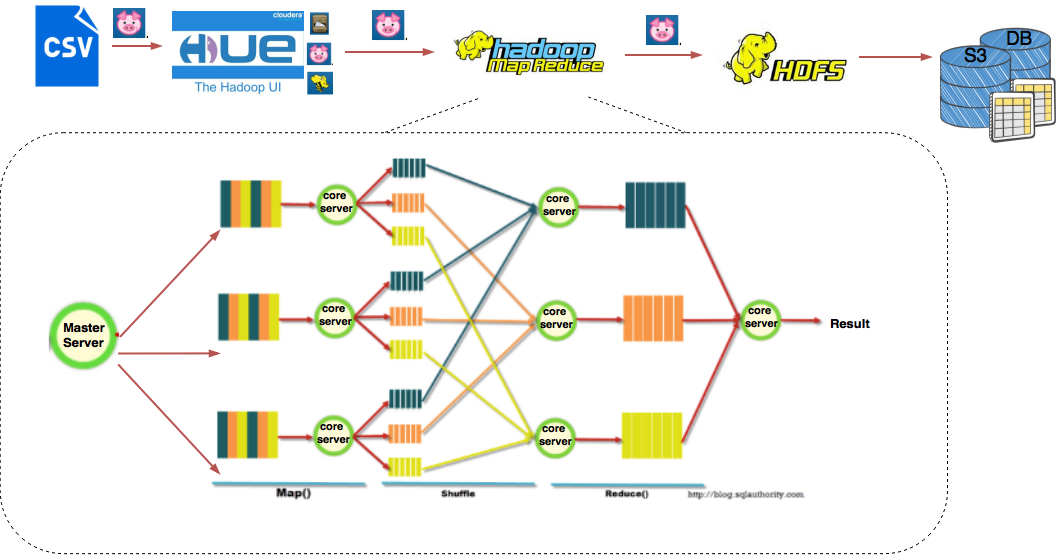
\includegraphics[width=2\columnwidth]{/Users/MariaFerman/Desktop/FinalReport/images/pigDiagram}
		\caption{Pig Diagram: shows the data process path of Pig}
		\label{fig:dataDiagr1}
	\end{center}
	\vspace{-10pt}
%\end{figure}
\end{figure*}

%\begin{figure}[H]
%\begin{figure*}[H]
	%\begin{center}
		%\includegraphics[width=2\columnwidth]{/Users/MariaFerman/Desktop/DC_FinalProject/images/HiveDiagram-2}
		%\caption{Hive Diagram}
		%\label{fig:dataDiagr2}
	%\end{center}
	%\vspace{-10pt}
%\end{figure}
%\end{figure*}

%\begin{figure}[H]
\begin{figure*}[H]
	\begin{center}
		\includegraphics[width=2\columnwidth]{/Users/MariaFerman/Desktop/FinalReport/images/HiveDiagram-2}
		\caption{Hive Diagram: shows the data process path of Hive.}
		\label{fig:dataDiagr3}
	\end{center}
	\vspace{-10pt}
%\end{figure}
\end{figure*}